%% Machine Learning and Agentic AI for Macroeconomic Research
%% Lecture 1: What is Quantitative Macroeconomics?
%% Author: Zhigang Feng
%% Based on: 1-2_intro/Lec_2026_2_quant_macro.tex

\documentclass[10pt,english,aspectratio=169]{beamer}

\usepackage{ae,aecompl}
\usepackage[T1]{fontenc}
\usepackage{textcomp}
\usepackage[utf8]{inputenc}
\usepackage{babel}

\setcounter{secnumdepth}{3}
\setcounter{tocdepth}{3}

\usepackage{amsmath, amssymb, graphicx}
\usepackage{booktabs, multirow}
\usepackage{tikz}
\usepackage{listings}
\usepackage{xcolor}

\lstset{
  basicstyle=\ttfamily\small,
  keywordstyle=\color{blue!80!black}\bfseries,
  commentstyle=\color{green!50!black}\itshape,
  stringstyle=\color{orange!80!black},
  backgroundcolor=\color{gray!8},
  frame=single,
  rulecolor=\color{gray!40},
  breaklines=true,
  showstringspaces=false,
  numbers=none,
}

\ifx\hypersetup\undefined
  \AtBeginDocument{%
    \hypersetup{bookmarks=false,breaklinks=true,pdfborder={0 0 0},colorlinks=true,
      linkcolor=DarkText,urlcolor=RedTitle}%
  }
\else
  \hypersetup{bookmarks=false,breaklinks=true,pdfborder={0 0 0},colorlinks=true,
    linkcolor=DarkText,urlcolor=RedTitle}%
\fi

\makeatletter
\newcommand\makebeamertitle{\frame{\maketitle}}%
\AtBeginDocument{%
  \let\origtableofcontents=\tableofcontents
  \def\tableofcontents{\@ifnextchar[{\origtableofcontents}{\gobbletableofcontents}}
  \def\gobbletableofcontents#1{\origtableofcontents}%
}

\usetheme{metropolis}
\usefonttheme{professionalfonts}

\definecolor{LightGray}{RGB}{230,230,230}
\definecolor{RedTitle}{RGB}{0,0,200}
\definecolor{VeryLightGray}{RGB}{245,245,245}
\definecolor{DarkText}{RGB}{0,0,0}

\setbeamercolor{background canvas}{bg=white}
\setbeamercolor{title}{fg=RedTitle}
\setbeamercolor{author}{fg=DarkText}
\setbeamercolor{date}{fg=DarkText}
\setbeamercolor{frametitle}{bg=VeryLightGray,fg=DarkText}
\setbeamercolor{normal text}{fg=DarkText}

\setbeamersize{text margin left=5mm, text margin right=5mm}
\addtobeamertemplate{frametitle}{}{\vspace{-0.5em}}
\newcommand{\reducevspace}{\vspace{-0.5cm}}

\setbeamertemplate{navigation symbols}{}
\setbeamertemplate{footline}{%
  \hfill%
  \usebeamercolor[fg]{page number in head/foot}%
  \usebeamerfont{page number in head/foot}%
  \insertframenumber\,/\,\inserttotalframenumber\kern1em\vskip2pt%
}

\makeatother

% Point figure includes back to original folder
\graphicspath{{../../1-2_intro/}}

\title[ML \& Agentic AI for Macro Research]{Machine Learning and Agentic AI for Macroeconomic Research\\
1: What is Quantitative Macroeconomics?\\[0.5em]}
\author{Zhigang Feng}
\date{Spring 2026}

\begin{document}

\makebeamertitle

%=============================================================================
% AGENDA
%=============================================================================

\begin{frame}{Lecture Agenda}
\begin{enumerate}
  \item \textbf{What is Quantitative Macroeconomics?}
    --- the field, workhorse models, methodological triad
  \medskip
  \item \textbf{The Optimal Growth Model}
    --- recursive formulation, Bellman equation, theoretical foundations
  \medskip
  \item \textbf{Two Constructive Approaches}
    --- Value function iteration (VFI) and Euler equation iteration
  \medskip
  \item \textbf{Heterogeneous Agent Models}
    --- Aiyagari, Krusell-Smith, infinite-dimensional state space
  \medskip
  \item \textbf{Theoretical Challenges}
    --- existence, uniqueness, curse of dimensionality
  \medskip
  \item \textbf{Calibration, Estimation, and Accuracy}
    --- mapping models to data, measuring solution quality
  \medskip
  \item \textbf{Bridge to AI/ML}
    --- why modern problems require new tools; course preview
\end{enumerate}
\end{frame}

%=============================================================================
% PART I: INTRODUCTION AND OVERVIEW
%=============================================================================

\section{What is Quantitative Macroeconomics?}

\begin{frame}{What is Quantitative Macroeconomics?}
\begin{itemize}
\item A field that uses numerical methods and computational tools to solve and analyze macroeconomic models, providing precise, quantitative answers to economic questions.

\medskip
\item \textbf{The Methodological Triad:}
\begin{enumerate}
    \item \emph{Theory:} Economic models with microfoundations
    \item \emph{Data:} Calibration and estimation
    \item \emph{Computation:} Numerical solution methods
\end{enumerate}

\medskip
\item \textbf{Core Techniques:}
\begin{itemize}
    \item Dynamic programming and optimal control
    \item Numerical optimization and root-finding
    \item Monte Carlo simulation
\end{itemize}

\medskip
\item \textbf{This Course:} Adding machine learning to the toolkit---neural networks, stochastic optimization, and deep reinforcement learning.
\end{itemize}
\end{frame}

\begin{frame}{What is Quantitative Macroeconomics?}
\begin{center}

\includegraphics[width=12cm,height=8cm]{pic/quant}
\par\end{center}
\end{frame}

\begin{frame}{Workhorse Models in Quantitative Macro}
\begin{itemize}
\item \textbf{Representative Agent Models:}
\begin{itemize}
    \item Neoclassical (stochastic) optimal growth model
    \item Real Business Cycle (RBC) model
    \item New Keynesian DSGE model
\end{itemize}

\medskip
\item \textbf{Heterogeneous Agent Models:}
\begin{itemize}
    \item Bewley-Aiyagari-Huggett (incomplete markets, idiosyncratic risk)
    \item Krusell-Smith (aggregate uncertainty + heterogeneity)
    \item Overlapping generations (OLG) models
\end{itemize}

\medskip
\item \textbf{Optimal Policy Models:}
\begin{itemize}
    \item Ramsey taxation problems
    \item Time-inconsistency and commitment
\end{itemize}

\medskip
\item \textbf{Common Thread:} All require solving dynamic optimization problems---the Bellman equation is central.
\end{itemize}
\end{frame}

%=============================================================================
% PART II: THE OPTIMAL GROWTH MODEL
%=============================================================================

\begin{frame}{Optimal Growth Model at the Core}
\begin{center}

\includegraphics[width=12cm,height=8cm]{pic/neocextension}
\par\end{center}
\end{frame}

\begin{frame}{Optimal Growth Model: Setup}
\begin{itemize}
\item The household solves the following dynamic optimization problem:
\begin{gather*}
\max_{\left\{ c_{t},k_{t+1}\right\} _{t=0}^{\infty}}\sum_{t=0}^{\infty}\beta^{t}\log c_{t} \\
\text{s.t. } c_{t}+k_{t+1}=Ak_{t}^{\alpha}+(1-\delta)k_{t}
\end{gather*}
\[
\beta\in(0,1),\quad A>0,\quad \alpha\in(0,1),\quad \delta\in[0,1]
\]
\[
k_{t}, c_{t}\geq0,\quad k_{0}\text{ given}, \quad t=0,1,2,\dots
\]
\item \textbf{Recursive Formulation (Bellman Equation):}
\[
v(k)=\max_{k' \in \Gamma(k)}\left\{ \log\left(Ak^{\alpha}+(1-\delta)k - k'\right)+\beta v(k') \right\}
\]
where $\Gamma(k) := \left\{ k' \mid 0 \leq k' \leq Ak^{\alpha}+(1-\delta)k \right\}$
\item \textbf{Solution:} Value function $v(k)$ and policy function $k'=g(k)$.
\end{itemize}
\end{frame}

\begin{frame}{From Sequence Problem to Recursive Problem}
\begin{itemize}
\item \textbf{The Challenge:} The sequence problem requires choosing an infinite sequence $\{c_t, k_{t+1}\}_{t=0}^{\infty}$ simultaneously---computationally intractable.

\medskip
\item \textbf{Key Insight:} The problem has \emph{recursive structure}---optimal decisions depend only on the current state $k$, not on history or calendar time.

\medskip
\item \textbf{Bellman's Principle of Optimality (1957):}
\begin{quote}
``An optimal policy has the property that whatever the initial state and initial decision are, the remaining decisions must constitute an optimal policy with regard to the state resulting from the first decision.''
\end{quote}

\medskip
\item \textbf{Implication:} Replace infinite-dimensional optimization with a functional equation---the Bellman equation---reducing the problem to finding a fixed point in function space.
\end{itemize}
\end{frame}

\section{Dynamic Programming Foundations}

\begin{frame}{The Bellman Operator}
\begin{itemize}
\item Define the \textbf{Bellman operator} $T: \mathcal{C}(X) \to \mathcal{C}(X)$:
\[
(Tv)(k) = \max_{k' \in \Gamma(k)}\left\{ u\left(Ak^{\alpha}+(1-\delta)k - k'\right)+\beta v(k') \right\}
\]

\medskip
\item The value function $v^*$ is a \textbf{fixed point}: $Tv^* = v^*$

\medskip
\item \textbf{Central Questions:}
\begin{enumerate}
    \item Does a fixed point exist?
    \item Is it unique?
    \item Can we compute it via iteration $v_{n+1} = Tv_n$?
    \item What properties does $v^*$ inherit (continuity, concavity)?
\end{enumerate}

\medskip
\item The following theoretical results answer these questions affirmatively.
\end{itemize}
\end{frame}

%=============================================================================
% PART III: THEORETICAL FOUNDATIONS
%=============================================================================

\begin{frame}{Contraction Mapping Theorem}
\begin{itemize}
\item \textbf{Definition:} Let $(S, d)$ be a metric space. An operator $T: S \to S$ is a \emph{contraction} with modulus $\beta \in (0,1)$ if:
\[
d(Tv, Tw) \leq \beta \cdot d(v, w) \quad \forall\, v, w \in S
\]

\medskip
\item \textbf{Contraction Mapping Theorem (Banach, 1922):} If $(S,d)$ is a complete metric space and $T$ is a contraction, then:
\begin{enumerate}
    \item $T$ has a \emph{unique} fixed point $v^* \in S$
    \item For any $v_0 \in S$, the sequence $v_{n+1} = Tv_n$ converges to $v^*$
    \item Rate of convergence: $d(v_n, v^*) \leq \frac{\beta^n}{1-\beta} d(v_1, v_0)$
\end{enumerate}

\medskip
\item \textbf{For Economics:} Guarantees that Value Function Iteration (VFI) converges to the unique solution of the Bellman equation.
\end{itemize}
\end{frame}

\begin{frame}{Blackwell's Sufficient Conditions}
\begin{itemize}
\item \textbf{Problem:} How do we verify that $T$ is a contraction?

\medskip
\item \textbf{Blackwell (1965):} An operator $T: \mathcal{B}(X) \to \mathcal{B}(X)$ on bounded functions is a contraction if:
\begin{enumerate}
    \item \textbf{Monotonicity:} $v(x) \leq w(x)$ for all $x$ $\Rightarrow$ $(Tv)(x) \leq (Tw)(x)$
    \item \textbf{Discounting:} $\exists\, \beta \in (0,1)$ such that $T(v + a)(x) \leq (Tv)(x) + \beta a$ for all $a \geq 0$
\end{enumerate}

\medskip
\item \textbf{Verification for the Bellman Operator:}
\begin{itemize}
    \item Monotonicity: Higher continuation value $\Rightarrow$ higher current value
    \item Discounting: The factor $\beta$ in $\beta v(k')$ provides the discounting
\end{itemize}

\medskip
\item \textbf{Key Insight:} The discount factor $\beta < 1$ is not just economically meaningful---it is mathematically essential for convergence.
\end{itemize}
\end{frame}

\begin{frame}{Theorem of the Maximum}
\begin{itemize}
\item \textbf{Theorem (Berge, 1963):} Let $f(x, a)$ be continuous and $\Gamma(x)$ be a continuous, compact-valued correspondence. Then:
\begin{enumerate}
    \item The \emph{value function} $v^*(x) = \max_{a \in \Gamma(x)} f(x,a)$ is continuous
    \item The \emph{policy correspondence} $G(x) = \arg\max_{a \in \Gamma(x)} f(x,a)$ is upper hemi-continuous
\end{enumerate}

\medskip
\item \textbf{Economic Implications:}
\begin{itemize}
    \item Small changes in $k$ lead to small changes in $v(k)$ and $g(k)$
    \item Ensures stability of computed solutions
    \item Justifies numerical approximation on discrete grids
\end{itemize}

\medskip
\item \textbf{Additional Properties:} Under strict concavity of $u(\cdot)$:
\begin{itemize}
    \item Policy correspondence is single-valued: a \emph{function} $g(k)$
    \item Value function $v(k)$ is strictly concave
\end{itemize}
\end{itemize}
\end{frame}

\begin{frame}{Theoretical Foundation: Summary}
\begin{center}
\begin{tabular}{l l}
\toprule
\textbf{Result} & \textbf{What It Guarantees} \\
\midrule
Principle of Optimality & Recursive formulation is valid \\
Contraction Mapping Thm & Existence, uniqueness, convergence \\
Blackwell's Conditions & Easy verification of contraction \\
Theorem of the Maximum & Continuity and stability \\
\bottomrule
\end{tabular}
\end{center}

\bigskip
\textbf{Together, these results establish:}
\begin{enumerate}
    \item The Bellman equation has a \emph{unique} solution $v^*$
    \item We can \emph{compute} $v^*$ by iterating $v_{n+1} = Tv_n$
    \item The solution is \emph{well-behaved} (continuous, concave)
    \item The policy function $g(k)$ is \emph{stable} under perturbations
\end{enumerate}

\bigskip
$\Rightarrow$ \textbf{Solid foundation for computational methods}
\end{frame}

%=============================================================================
% PART IV: COMPETITIVE EQUILIBRIUM AND RECURSIVE FORMULATION
%=============================================================================

\section{Equilibrium Concepts}

\begin{frame}{Competitive Equilibrium: Definition}
\begin{itemize}
\item \textbf{A competitive equilibrium} consists of:
\begin{enumerate}
    \item \emph{Prices:} $\{r_t, w_t\}_{t=0}^\infty$ (rental rate and wage)
    \item \emph{Allocations:} $\{c_t, k_{t+1}, n_t\}_{t=0}^\infty$
\end{enumerate}
such that: (i) households optimize, (ii) firms optimize, (iii) markets clear.

\medskip
\item \textbf{Key Equilibrium Conditions:}
\begin{itemize}
    \item Factor prices: $r_t = \alpha A k_t^{\alpha-1} - \delta$, \quad $w_t = (1-\alpha)A k_t^\alpha$
    \item Household Euler equation: $u'(c_t) = \beta \mathbb{E}_t[u'(c_{t+1})(1 + r_{t+1})]$
    \item Resource constraint: $c_t + k_{t+1} = A k_t^\alpha + (1-\delta)k_t$
\end{itemize}

\medskip
\item \textbf{Recursive (Markov) Equilibrium:} An equilibrium where decisions depend only on \emph{payoff-relevant} state variables, not on calendar time or history.
\begin{itemize}
    \item Representative agent: state = $(k, z)$
    \item Policy rules: $c = \sigma(k,z)$, $k' = g(k,z)$, prices $r = r(k,z)$, $w = w(k,z)$
\end{itemize}
\end{itemize}
\end{frame}

\begin{frame}{From Competitive Equilibrium to Social Planner}
\begin{itemize}
\item \textbf{First Welfare Theorem:} Under complete markets and no externalities, a competitive equilibrium is Pareto optimal.

\medskip
\item \textbf{Implication for Computation:}
\begin{itemize}
    \item For representative agent models, solve the social planner's problem
    \item Recover prices from planner's marginal conditions
    \item Avoids fixed-point problem over prices
\end{itemize}

\medskip
\item \textbf{When the Theorem Fails:}
\begin{itemize}
    \item Incomplete markets (Aiyagari, Bewley): no Pareto optimality
    \item Externalities, taxes, monopolistic competition
    \item Must solve for equilibrium prices \emph{explicitly}
\end{itemize}

\medskip
\item \textbf{Practical Implication:}
\begin{itemize}
    \item Representative agent models: ``easy'' (solve planner's problem)
    \item Heterogeneous agent models: ``hard'' (must iterate on distribution + prices)
\end{itemize}
\end{itemize}
\end{frame}

%=============================================================================
% PART V: TWO CONSTRUCTIVE APPROACHES
%=============================================================================

\begin{frame}{Two Roads to Equilibrium}
\begin{itemize}
\item We have two constructive algorithms for computing equilibrium:

\bigskip
\item \textbf{Approach 1: Dynamic Programming (Value Function Iteration)}
\begin{itemize}
    \item Iterate on the Bellman equation: $v_{n+1} = Tv_n$
    \item Convergence via \emph{contraction mapping}
    \item Recovers both value function and policy
\end{itemize}

\bigskip
\item \textbf{Approach 2: Euler Equation Iteration (Greenwood-Huffman)}
\begin{itemize}
    \item Iterate directly on the policy function via Euler equation
    \item Convergence via \emph{monotonicity}
    \item Works directly with equilibrium conditions
\end{itemize}

\bigskip
\item Both approaches are \emph{constructive}---they provide algorithms, not just existence proofs.
\end{itemize}
\end{frame}

\section{Two Classical Approaches}

\begin{frame}{Dynamic Programming: The Classical Framework}
\begin{itemize}
\item \textbf{Dynamic Programming (Bellman, 1957):} Solve sequential decision problems by exploiting recursive structure.

\medskip
\item \textbf{Core Idea:} Value of any state = max over (immediate reward + discounted continuation):
\[
v(s) = \max_{a \in \Gamma(s)} \left\{ r(s, a) + \beta \, \mathbb{E}\left[ v(s') \mid s, a \right] \right\}
\]

\medskip
\item \textbf{Value Function Iteration (VFI):}
\begin{enumerate}
    \item Discretize state space into finite grid $\{s_1, \ldots, s_N\}$
    \item Initialize $v_0(s_i)$ for each grid point
    \item Iterate: $v_{n+1}(s_i) = \max_{a} \{ r(s_i, a) + \beta \sum_j P(s_j|s_i,a) v_n(s_j) \}$
    \item Stop when $\|v_{n+1} - v_n\| < \varepsilon$
\end{enumerate}

\medskip
\item \textbf{Requirement:} Complete knowledge of the environment---$P(s'|s,a)$ and $r(s,a)$.
\end{itemize}
\end{frame}

\begin{frame}{Euler Equation Approach: Setup}
\begin{itemize}
\item \textbf{Alternative:} Work directly with first-order conditions (Euler equations).

\medskip
\item The Euler equation for the optimal growth model:
\[
u'(c_t) = \beta \, \mathbb{E}_t \left[ u'(c_{t+1}) \cdot F_k(k_{t+1}, z_{t+1}) \right]
\]

\medskip
\item In a competitive equilibrium with $k = K$:
\begin{multline*}
u_c(c(k,K,k',z)) = \\
\beta \, \mathbb{E} \left[ u_c(c(k',K',k'',z')) \cdot F_k(k',K',z') \mid z \right]
\end{multline*}

\medskip
\item \textbf{Equilibrium Requirement:} Find policy $g$ and aggregate law of motion $G$ such that:
\begin{itemize}
    \item The Euler equation holds for all $(k, K, z)$
    \item Consistency: $G(K, z) = g(K, K, z)$ (individual = aggregate)
\end{itemize}
\end{itemize}
\end{frame}

\begin{frame}{The Greenwood-Huffman Operator}
\begin{itemize}
\item \textbf{Idea:} Construct a sequence of policy functions that converges to equilibrium.

\medskip
\item Let $H^{0}(K,z) = 0$. Define $H^{j+1}(K,z)$ as the $x$ solving:
\[
u_c(c(K,K,x,z)) = \beta \, \mathbb{E} \left[ u_c(c(x,x,H^{j}(x,z'),z')) \cdot F_k(x,x,z') \right]
\]

\medskip
\item \textbf{Interpretation:}
\begin{itemize}
    \item Given a conjecture $H^j$ for future policy, solve for today's optimal $x$
    \item The solution $x = H^{j+1}(K,z)$ becomes the new conjecture
    \item Iterate until convergence: $H^{j+1} \approx H^j$
\end{itemize}

\medskip
\item \textbf{Convergence via Monotonicity:}
\begin{itemize}
    \item $\{H^j\}$ is monotone (increasing from $H^0 = 0$)
    \item Bounded by resource constraint $H^j(K,z) \leq F(K,K,z)$
    \item Monotone + bounded $\Rightarrow$ limit $H^*$ exists
\end{itemize}
\end{itemize}
\end{frame}

\begin{frame}{Comparing the Two Approaches}
\begin{center}
\renewcommand{\arraystretch}{1.3}
\begin{tabular}{|l|c|c|}
\hline
 & \textbf{Value Function Iteration} & \textbf{Euler Equation Iteration} \\
\hline
\textbf{Object} & Value function $v(k)$ & Policy function $H(K,z)$ \\
\textbf{Iteration} & $v_{n+1} = Tv_n$ & $H^{j+1} = TH^j$ \\
\textbf{Convergence} & Contraction & Monotonicity \\
\textbf{Theory} & Banach fixed point & Monotone convergence \\
\hline
\textbf{Strength} & General, robust & Direct equilibrium \\
\textbf{Weakness} & Indirect (need to extract $g$) & Requires monotonicity \\
\hline
\end{tabular}
\end{center}

\bigskip
\textbf{Both provide:}
\begin{itemize}
    \item Constructive algorithms (not just existence proofs)
    \item Theoretical guarantees for convergence
    \item Foundation for numerical implementation
\end{itemize}
\end{frame}

%=============================================================================
% PART VI: WHY REPRESENTATIVE AGENT MODELS ARE "EASY"
%=============================================================================

\begin{frame}{Why Classical Macro Models Are ``Easy''}
\begin{itemize}
\item \textbf{Representative Agent + First Welfare Theorem:}
\begin{itemize}
    \item Competitive equilibrium $\Leftrightarrow$ Social planner's solution
    \item No need to explicitly compute prices to find allocations
\end{itemize}

\medskip
\item \textbf{The Key Simplification:} Individual capital $k$ = Aggregate capital $K$
\begin{itemize}
    \item Prices are deterministic functions of a single state variable:
    \[
    r(K) = \alpha A K^{\alpha - 1} - \delta, \qquad w(K) = (1-\alpha) A K^{\alpha}
    \]
    \item The agent \emph{knows} how prices evolve because $K' = g(K)$
\end{itemize}

\medskip
\item \textbf{By Design, Not by Accident:}
\begin{itemize}
    \item Economists constructed this framework for tractability
    \item The ``environment'' is fully specified by $(A, \alpha, \beta, \delta)$
    \item State space is low-dimensional (often just $k$ or $(k, z)$)
\end{itemize}
\end{itemize}
\end{frame}

%=============================================================================
% PART VII: HETEROGENEOUS AGENT MODELS
%=============================================================================

\section{Model Extensions and Challenges}

\begin{frame}{Extensions Based on the Optimal Growth Model}
\begin{center}

\includegraphics[width=12cm,height=8cm]{pic/neoclastruct}
\par\end{center}
\end{frame}

\begin{frame}{Heterogeneous Agents: Breaking the Simplicity}
\begin{itemize}
\item \textbf{Realistic Extension:} Agents differ in wealth, income, productivity
\begin{itemize}
    \item Individual state: $(a_i, z_i)$ --- assets and idiosyncratic shock
    \item Now $k_i \neq K$; individual choices don't reveal aggregates
\end{itemize}

\medskip
\item \textbf{Prices Depend on the Distribution:}
\[
r = r(\mu), \qquad w = w(\mu)
\]
where $\mu$ is the \emph{cross-sectional distribution} of $(a, z)$

\medskip
\item \textbf{The Distribution Is a State Variable:}
\begin{itemize}
    \item To forecast prices, agents must forecast how $\mu$ evolves
    \item But $\mu$ is \emph{infinite-dimensional}---a measure over $(a, z)$
    \item Evolution: $\mu' = \Phi(\mu; g)$ depends on everyone's policy
\end{itemize}

\medskip
\item \textbf{The Environment Is No Longer Obvious:}
\begin{itemize}
    \item Agents face a \emph{perceived law of motion} they must approximate
    \item First Welfare Theorem fails $\Rightarrow$ must solve for prices explicitly
\end{itemize}
\end{itemize}
\end{frame}

\begin{frame}{Bewley-Aiyagari-Huggett Model}
\begin{itemize}
\item \textbf{Setup:}
\begin{itemize}
    \item Continuum of infinitely lived households (measure 1)
    \item Uninsurable idiosyncratic income shocks $\epsilon$
    \item \emph{Ex-ante} identical, \emph{ex-post} heterogeneous
\end{itemize}

\medskip
\item \textbf{Bellman Equation:}
\[
v(a,\epsilon;\lambda)=\max_{c,a'}\left\{ u(c)+\beta\sum_{\epsilon'}v(a',\epsilon';\lambda')\pi(\epsilon,\epsilon') \right\}
\]
subject to:
\begin{align*}
c+a' & = (1+r(\lambda))a+w(\lambda)\epsilon \\
a' & \geq -\underline{a}
\end{align*}

\medskip
\item \textbf{Stationary Equilibrium:} Find $\lambda^*$ such that $\lambda^* = \Phi(\lambda^*; g)$
\begin{itemize}
    \item Distribution is invariant under optimal policies
    \item Incomplete markets endogenously generate wealth inequality
\end{itemize}
\end{itemize}
\end{frame}

\begin{frame}{Krusell-Smith Model}
\begin{itemize}
\item \textbf{Extension:} Add \emph{aggregate uncertainty} to Aiyagari

\medskip
\item \textbf{Aggregate shock:} $z_t \in \{z_g, z_b\}$ (good/bad states)
\begin{itemize}
    \item Affects aggregate productivity
    \item Unemployment higher in bad states: $u_b > u_g$
\end{itemize}

\medskip
\item \textbf{Household Problem:}
\[
v(k,\epsilon;\Gamma,z)=\max_{c,k'} \left\{ U(c)+\beta \, \mathbb{E}[v(k',\epsilon';\Gamma',z') \mid z,\epsilon] \right\}
\]
subject to:
\begin{align*}
c+k' &= r(\bar{k},\bar{l})k + w(\bar{k},\bar{l})\epsilon + (1-\delta)k \\
\Gamma' &= H(\Gamma,z,z'), \qquad k' \geq 0
\end{align*}

\medskip
\item \textbf{The Challenge:} Agents must forecast evolution of $\Gamma$---infinite-dimensional!
\end{itemize}
\end{frame}

\begin{frame}{Krusell-Smith: The Computational Innovation}
\begin{itemize}
\item \textbf{Key Insight (Krusell-Smith, 1998):}
\begin{itemize}
    \item Agents don't need to track the entire distribution $\Gamma$
    \item Approximate with low-dimensional moments: $\bar{K} = \int k \, d\Gamma$
\end{itemize}

\medskip
\item \textbf{Bounded Rationality:} Agents use simple forecasting rules
\[
\log \bar{K}' = a_0(z) + a_1(z) \log \bar{K}
\]

\medskip
\item \textbf{Algorithm:}
\begin{enumerate}
    \item Guess coefficients $(a_0, a_1)$
    \item Solve individual problem given forecasting rule
    \item Simulate economy, regress $\log \bar{K}'$ on $\log \bar{K}$
    \item Update coefficients; iterate until convergence
\end{enumerate}

\medskip
\item \textbf{Remarkable Finding:} $R^2 > 0.999$---mean capital is nearly sufficient!
\end{itemize}
\end{frame}

%=============================================================================
% PART VIII: THEORETICAL CHALLENGES
%=============================================================================

\begin{frame}{Theoretical Issues in Heterogeneous Agent Models}
\begin{itemize}
\item \textbf{Existence of Recursive Equilibrium:}
\begin{itemize}
    \item When markets are complete/efficient: easier to prove
    \item Incomplete markets: may require forward-looking variables
\end{itemize}

\medskip
\item \textbf{Uniqueness:} Generally \emph{not} guaranteed
\begin{itemize}
    \item Multiple steady states possible
    \item Policy functions may have discontinuities
\end{itemize}

\medskip
\item \textbf{Continuity:} Value and policy functions may not be continuous in aggregates

\medskip
\item \textbf{Computation:}
\begin{itemize}
    \item Curse of dimensionality (distribution as state)
    \item Ensuring accuracy of approximations
    \item Verifying equilibrium conditions
\end{itemize}

\medskip
\item \textbf{These issues become more severe in optimal policy (Ramsey) problems.}
\end{itemize}
\end{frame}

\begin{frame}{Example: Non-Existence of Continuous Equilibrium}
\textbf{Santos (2002):} Representative household, $\sum \beta^t \log(c_t)$, subject to:
\[
c_{t}+k_{t+1} \leq \pi_{t}+(1-\tau_{t})r_{t}k_{t}+T_{t}
\]
with piecewise linear tax on capital:
\[
\tau(K) = \begin{cases}
0.10 & \text{if } K \leq 0.160 \\
0.05 - 10(K - 0.165) & \text{if } 0.160 < K < 0.170 \\
0 & \text{if } K \geq 0.170
\end{cases}
\]

\medskip
\textbf{Result:} A continuous Markov equilibrium \emph{fails to exist}.
\begin{itemize}
    \item Middle steady state: unstable (complex eigenvalues)
    \item Other steady states: saddle-path stable
    \item Equilibrium exhibits cycles or discontinuities
\end{itemize}
\end{frame}

\begin{frame}{Theoretical Issues: Equilibrium Cycles}
\begin{center}

\includegraphics[width=11cm,height=7cm]{pic/cycle_compare}
\par\end{center}
\end{frame}

\begin{frame}{Ramsey Problem: Additional State Variables}
\begin{itemize}
\item \textbf{Consumer FOCs:}
\begin{itemize}
    \item Consumption: $\lambda_{t}=u_{c_t}$
    \item Labor: $u_{n}=(1-\tau_{t})u_{c}f_{n}$
    \item Euler: $\lambda_{t}=\lambda_{t+1}\beta[(1-\theta_{t+1})f_{k}+1-\delta]$
\end{itemize}

\medskip
\item \textbf{The Problem:} Euler equation can be rewritten backward:
\[
\lambda_{t-1}=\lambda_{t}\beta[(1-\theta_{t})f_{k}(k_{t},n_{t})+1-\delta]
\]

\medskip
\item \textbf{Implication:} Must track $\lambda_{t-1}$ as a state variable
\begin{itemize}
    \item Minimal state space $(k_t)$ is \emph{insufficient}
    \item Need $(k_t, \lambda_{t-1})$ with unknown domain for $\lambda$
\end{itemize}

\medskip
\item \textbf{Consequence:} State space expands; recursive formulation becomes more complex.
\end{itemize}
\end{frame}

%=============================================================================
% PART IX: THE CURSE OF DIMENSIONALITY
%=============================================================================

\begin{frame}{The Curse of Dimensionality}
\begin{itemize}
\item \textbf{Bellman (1961):} Named the ``curse of dimensionality''---exponential growth of computational cost with state dimension.

\medskip
\item \textbf{Grid-Based Methods:}
\begin{itemize}
    \item $n$ grid points per dimension, $d$ dimensions $\Rightarrow$ $n^d$ total points
    \item Example: 100 points $\times$ 10 dimensions = $10^{20}$ points
    \item Infeasible for storage, let alone computation
\end{itemize}

\medskip
\item \textbf{Heterogeneous Agent Models:}
\begin{itemize}
    \item Distribution $\mu$ is infinite-dimensional
    \item Even discretized: thousands of $(a, z)$ pairs $\times$ aggregate states
    \item Standard VFI becomes computationally prohibitive
\end{itemize}

\medskip
\item \textbf{This is exactly the challenge AI/RL research confronts}---in even more extreme settings.
\end{itemize}
\end{frame}

%=============================================================================
% PART X: NUMERICAL METHODS
%=============================================================================

\begin{frame}{Numerical Methods: Interpolation and Approximation}
\begin{itemize}
\item \textbf{Purpose:} Represent value and policy functions on a computer.

\medskip
\item \textbf{Interpolation Methods:}
\begin{itemize}
    \item \emph{Linear interpolation:} Simple, fast, not smooth
    \item \emph{Cubic splines:} Smooth, accurate for smooth functions
    \item \emph{Chebyshev polynomials:} Near-optimal approximation on $[-1,1]$; avoid Runge's phenomenon
\end{itemize}

\medskip
\item \textbf{Discretization of Stochastic Processes:}
\begin{itemize}
    \item \emph{Tauchen (1986):} Discretize AR(1) $z_t = \rho z_{t-1} + \sigma \varepsilon_t$ via finite Markov chain
    \item \emph{Rouwenhorst (1995):} Better for highly persistent processes ($\rho \approx 1$)
\end{itemize}

\medskip
\item \textbf{Projection Methods:}
\begin{itemize}
    \item Approximate $v(k) \approx \sum_j c_j \phi_j(k)$ using basis functions
    \item Choose coefficients to minimize residuals in Bellman equation
\end{itemize}
\end{itemize}
\end{frame}

\begin{frame}{Numerical Methods: Optimization}
\begin{itemize}
\item \textbf{Maximization in the Bellman Equation:}
\[
\max_{k' \in \Gamma(k)} \left\{ u(f(k) - k') + \beta v(k') \right\}
\]

\medskip
\item \textbf{Classical Methods:}
\begin{itemize}
    \item \emph{Grid search:} Evaluate objective at all grid points; pick max --- reliable but slow
    \item \emph{Golden section search:} Exploit unimodality; $O(\log n)$ evaluations
    \item \emph{Newton-Raphson:} Use derivatives for fast convergence; $O(\text{quadratic})$
\end{itemize}

\medskip
\item \textbf{Modern Methods:}
\begin{itemize}
    \item \emph{Automatic differentiation (PyTorch):} Exact gradients from code
    \item \emph{Stochastic gradient descent (SGD/Adam):} Scale to high dimensions
    \item \emph{Gradient-based optimization:} Essential for neural network training
\end{itemize}

\medskip
\item \textbf{Rule of Thumb:} Use derivatives when available; they dramatically speed up convergence.
\end{itemize}
\end{frame}

\begin{frame}{Numerical Methods: Simulation}
\begin{itemize}
\item \textbf{Monte Carlo Simulation:} Generate artificial time series from a calibrated model.

\medskip
\item \textbf{Algorithm:}
\begin{enumerate}
    \item Draw shocks $\{z_t\}_{t=1}^T$ from the Markov chain
    \item Given policy $g$, compute $k_{t+1} = g(k_t, z_t)$ and $c_t = f(k_t, z_t) - k_{t+1}$
    \item Compute moments: mean, variance, autocorrelation, cross-correlations
\end{enumerate}

\medskip
\item \textbf{Uses in Quantitative Macro:}
\begin{itemize}
    \item \emph{Calibration:} Match model moments to data moments
    \item \emph{Counterfactuals:} Study effects of policy changes
    \item \emph{Distribution computation:} Simulate agent distribution in HA models
\end{itemize}

\medskip
\item \textbf{Key Consideration:} Burn-in period; law of large numbers requires $T \to \infty$
\end{itemize}
\end{frame}

%=============================================================================
% PART XI: CALIBRATION, ESTIMATION, AND ACCURACY
%=============================================================================

\begin{frame}{Calibration: Mapping Models to Data}
\begin{itemize}
\item \textbf{Goal:} Choose model parameters $\theta = (\beta, \alpha, \delta, \sigma, \rho, \ldots)$ so the model matches key empirical regularities.

\medskip
\item \textbf{Calibration Strategies:}
\begin{enumerate}
    \item \emph{Direct calibration:} Match parameter to single data moment directly\\
        \quad e.g., $\alpha = $ labor share $\approx 0.36$; $\delta = $ depreciation rate $\approx 0.10$
    \item \emph{Indirect calibration:} Choose $\theta$ to minimize distance between model and data moments\\
        \quad e.g., $\beta$ calibrated to match capital-output ratio
    \item \emph{Steady-state calibration:} Use steady-state conditions as moment restrictions
\end{enumerate}

\medskip
\item \textbf{Typical Moments Targeted:}
\begin{itemize}
    \item Capital-output ratio, consumption-output ratio
    \item Labor share, average hours worked
    \item Volatility and autocorrelation of GDP, consumption, investment
    \item Cross-sectional wealth and income inequality
\end{itemize}
\end{itemize}
\end{frame}

\begin{frame}{Estimation: Formal Inference}
\begin{itemize}
\item \textbf{Calibration vs.\ Estimation:}
\begin{itemize}
    \item Calibration: informal, one-to-one moment matching
    \item Estimation: formal statistical framework, uncertainty quantification
\end{itemize}

\medskip
\item \textbf{Simulated Method of Moments (SMM):}
\[
\hat{\theta} = \arg\min_\theta \left[ m_{\text{data}} - m_{\text{model}}(\theta) \right]' W \left[ m_{\text{data}} - m_{\text{model}}(\theta) \right]
\]
where $W$ is a weighting matrix; accounts for estimation uncertainty.

\medskip
\item \textbf{Indirect Inference (Gourieroux et al., 1993):}
\begin{itemize}
    \item Fit auxiliary model to both data and simulated data
    \item Match the \emph{auxiliary model parameters}
    \item Useful when data has complex time-series structure
\end{itemize}

\medskip
\item \textbf{Bayesian Methods:}
\begin{itemize}
    \item Prior $p(\theta)$ + likelihood $p(\text{data}|\theta)$ $\Rightarrow$ posterior $p(\theta|\text{data})$
    \item MCMC sampling; popular for DSGE models
\end{itemize}
\end{itemize}
\end{frame}

\begin{frame}{Accuracy Analysis: How Good Is the Solution?}
\begin{itemize}
\item \textbf{Problem:} Numerical methods produce approximations. How do we measure quality?

\medskip
\item \textbf{Euler Equation Residuals (Judd, 1992):}
\[
\text{EEE}(k) = \left| 1 - \frac{\beta u'(c_{t+1}) F_k(k_{t+1}, z_{t+1})}{u'(c_t)} \right|
\]
\begin{itemize}
    \item Measures how well the computed policy satisfies optimality conditions
    \item Interpretation: fraction of consumption (``dollar unit'') wasted by approximation error
    \item Target: $|\text{EEE}| < 10^{-4}$ (less than 0.01\% error)
\end{itemize}

\medskip
\item \textbf{Den Haan-Marcet Test:} Statistical test for whether forecast errors are unpredictable --- checks if optimality conditions hold on average.

\medskip
\item \textbf{Policy Function Comparison:} Compare solution across methods (VFI, EGM, projection) to verify agreement.
\end{itemize}
\end{frame}

\begin{frame}{Perturbation Methods: Linearization}
\begin{itemize}
\item \textbf{Idea:} Approximate the equilibrium around the deterministic steady state.

\medskip
\item \textbf{First-Order Perturbation (Log-linearization):}
\[
\hat{x}_{t+1} \approx A \hat{x}_t + B \hat{z}_t
\]
where $\hat{x}_t = \log x_t - \log x^*$ are log-deviations from steady state.
\begin{itemize}
    \item Fast and tractable; the workhorse of DSGE estimation (Dynare)
    \item Ignores risk---agents behave as if the future is certain
\end{itemize}

\medskip
\item \textbf{Higher-Order Perturbation:}
\begin{itemize}
    \item 2nd order: captures precautionary saving, risk premia
    \item 3rd order: skewness, asymmetric responses to shocks
    \item Dramatically more complex, but still closed-form
\end{itemize}

\medskip
\item \textbf{Limitation:} Valid only near steady state; fails for large shocks or crises.
\end{itemize}
\end{frame}

%=============================================================================
% SUPPLEMENTARY RESOURCE
%=============================================================================

\begin{frame}{Supplementary Resource: Classical Numerical Methods}
\begin{tcolorbox}[colback=blue!3, colframe=blue!40, title=Video Lecture Series]
Complete recordings of classical computational methods for macroeconomists are available at:
\begin{center}
\url{https://space.bilibili.com/2142649036/lists/7180709}
\end{center}
\medskip
Topics include:
\begin{itemize}
  \item Numerical solution methods: value function iteration, time iteration
  \item Advanced methods: Howard improvement, endogenous grid method (EGM)
  \item Perturbation methods (first- and second-order)
  \item Projection methods: Chebyshev polynomials, collocation
  \item Numerical optimization, interpolation, and simulation
  \item High-performance and parallel computing (MPI, GPU)
\end{itemize}
\end{tcolorbox}
\end{frame}

%=============================================================================
% PART XII: BRIDGE TO AI/ML
%=============================================================================

\section{The AI/RL Alternative}

\begin{frame}{AI/Reinforcement Learning: The Robot-Taxi Problem}
\begin{itemize}
\item \textbf{Example:} Training an autonomous vehicle to navigate a city

\medskip
\item \textbf{State Space:} Camera images, LiDAR, GPS, speed, ...
\begin{itemize}
    \item Single camera frame: $1920 \times 1080 \times 3 \approx 6$ million dimensions
    \item Continuous, high-dimensional, partially observable
\end{itemize}

\medskip
\item \textbf{Action Space:} Steering, acceleration, braking (continuous)

\medskip
\item \textbf{Environment:} Transition dynamics $P(s'|s, a)$
\begin{itemize}
    \item Physics, other drivers, pedestrians, weather
    \item \emph{Unknown} and \emph{impossible to fully specify}
    \item No ``First Welfare Theorem'' to simplify
\end{itemize}

\medskip
\item \textbf{Contrast with Macro:} No closed-form model; must learn from experience
\end{itemize}
\end{frame}

\begin{frame}{RL Formulation: The Same Bellman Equation}
\begin{itemize}
\item \textbf{Markov Decision Process (MDP):} $(S, A, P, r, \beta)$

\medskip
\item \textbf{Bellman Equation for Optimal Value:}
\[
v^*(s) = \max_{a} \left\{ r(s, a) + \beta \int v^*(s') P(ds'|s, a) \right\}
\]

\medskip
\item \textbf{Bellman Equation for Q-Function:}
\[
Q^*(s, a) = r(s, a) + \beta \int \max_{a'} Q^*(s', a') P(ds'|s, a)
\]

\medskip
\item \textbf{Key Insight:} Theoretical foundation is \emph{identical} to economics.
\begin{itemize}
    \item Bellman equation, contraction mapping, fixed point---all apply
\end{itemize}

\medskip
\item \textbf{The difference is computational:} How do we solve this when $P$ is unknown and $S$ is enormous?
\end{itemize}
\end{frame}

\begin{frame}{Three Fundamental Challenges}
\begin{center}
\renewcommand{\arraystretch}{1.4}
\begin{tabular}{|c|c|c|}
\hline
\textbf{Challenge} & \textbf{Classical DP} & \textbf{Modern AI/RL} \\
\hline
\textbf{Dimensionality} & Low $(d \leq 5)$ & Very high $(d \geq 10^6)$ \\
\hline
\textbf{Environment} & Fully known & Unknown, learned \\
\hline
\textbf{Data} & Regular grids & Random samples \\
\hline
\end{tabular}
\end{center}

\bigskip
\begin{itemize}
\item \textbf{Dimensionality:} Cannot discretize; must use function approximation
\item \textbf{Unknown Environment:} Cannot evaluate $\mathbb{E}[v(s')]$ analytically; estimate from samples (Monte Carlo)
\item \textbf{Irregular Data:} Samples from trajectories, not grids; must generalize
\end{itemize}
\end{frame}

\begin{frame}{Monte Carlo: Turning Samples into Expectations}
\begin{itemize}
\item \textbf{The Problem:} Computing $\mathbb{E}[v(s') | s, a] = \int v(s') P(ds'|s, a)$
\begin{itemize}
    \item Classical DP: Enumerate all $s'$, weight by known $P(s'|s, a)$
    \item High dimensions or unknown $P$: Infeasible
\end{itemize}

\medskip
\item \textbf{Monte Carlo Estimation:}
\[
\mathbb{E}[v(s')] \approx \frac{1}{N} \sum_{i=1}^{N} v(s'_i), \qquad s'_i \sim P(\cdot | s, a)
\]
\begin{itemize}
    \item Generate samples by \emph{simulating} or \emph{interacting} with environment
    \item Law of Large Numbers: Converges as $N \to \infty$
\end{itemize}

\medskip
\item \textbf{Key Advantage:} Cost scales with $N$, \emph{not} dimension
\begin{itemize}
    \item Works equally well in 2 or 2 million dimensions
    \item This is how RL escapes the curse of dimensionality
\end{itemize}
\end{itemize}
\end{frame}

\begin{frame}{Function Approximation: Learning from Irregular Data}
\begin{itemize}
\item \textbf{Classical DP:} Value function as table $\{v(s_i)\}_{i=1}^{N}$
\begin{itemize}
    \item Regular grid, pre-specified, covers entire state space
    \item Interpolation straightforward
\end{itemize}

\medskip
\item \textbf{RL with Function Approximation:}
\[
v(s) \approx v_\theta(s) = \text{NeuralNetwork}_\theta(s)
\]
\begin{itemize}
    \item Parameters $\theta$ learned from sampled data
    \item Data from trajectories: $(s_0, a_0, r_0, s_1, a_1, r_1, \ldots)$
    \item Points concentrate where policy visits (not uniform)
\end{itemize}

\medskip
\item \textbf{Challenges:}
\begin{itemize}
    \item Must generalize to unseen states
    \item Approximation errors can compound (instability)
    \item No convergence guarantee (unlike tabular DP)
\end{itemize}
\end{itemize}
\end{frame}

\begin{frame}{From Grids to Samples: A Paradigm Shift}
\begin{center}
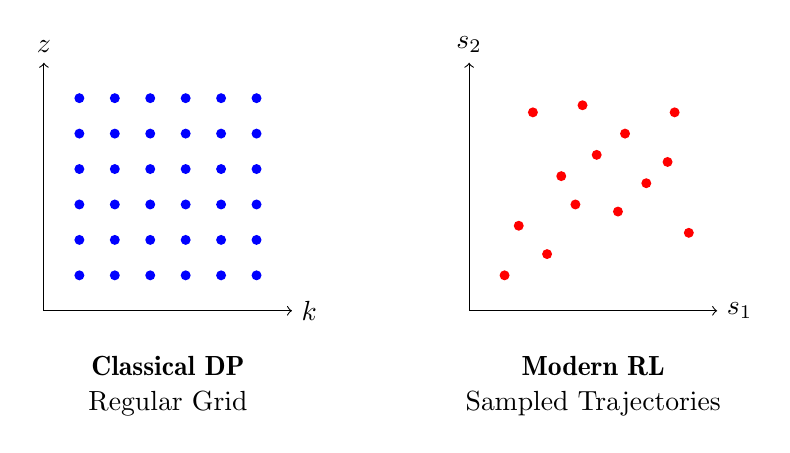
\begin{tikzpicture}[scale=0.9]
% Classical DP - Grid
\begin{scope}[shift={(-4,0)}]
\draw[->] (0,0) -- (3.5,0) node[right] {$k$};
\draw[->] (0,0) -- (0,3.5) node[above] {$z$};
\foreach \x in {0.5,1,1.5,2,2.5,3}
    \foreach \y in {0.5,1,1.5,2,2.5,3}
        \fill[blue] (\x,\y) circle (2pt);
\node[below] at (1.75,-0.5) {\textbf{Classical DP}};
\node[below] at (1.75,-1) {Regular Grid};
\end{scope}
% Modern RL - Random Samples
\begin{scope}[shift={(2,0)}]
\draw[->] (0,0) -- (3.5,0) node[right] {$s_1$};
\draw[->] (0,0) -- (0,3.5) node[above] {$s_2$};
\fill[red] (0.7,1.2) circle (2pt);
\fill[red] (1.1,0.8) circle (2pt);
\fill[red] (1.5,1.5) circle (2pt);
\fill[red] (1.3,1.9) circle (2pt);
\fill[red] (2.1,1.4) circle (2pt);
\fill[red] (1.8,2.2) circle (2pt);
\fill[red] (2.5,1.8) circle (2pt);
\fill[red] (2.2,2.5) circle (2pt);
\fill[red] (2.8,2.1) circle (2pt);
\fill[red] (0.9,2.8) circle (2pt);
\fill[red] (1.6,2.9) circle (2pt);
\fill[red] (2.9,2.8) circle (2pt);
\fill[red] (0.5,0.5) circle (2pt);
\fill[red] (3.1,1.1) circle (2pt);
\node[below] at (1.75,-0.5) {\textbf{Modern RL}};
\node[below] at (1.75,-1) {Sampled Trajectories};
\end{scope}
\end{tikzpicture}
\end{center}

\medskip
\begin{itemize}
\item \textbf{Left:} Compute $v(s)$ at every grid point; interpolate
\item \textbf{Right:} Observe $(s, a, r, s')$ tuples; fit $v_\theta(s)$ to minimize prediction error
\end{itemize}
\end{frame}

\begin{frame}{Heterogeneous Agent Models: Between Two Worlds}
\begin{itemize}
\item \textbf{Individual Problem:} Low-dimensional $(a, z)$---classical methods work
\item \textbf{Aggregate State:} Distribution $\mu$---infinite-dimensional

\medskip
\item \textbf{Traditional Approaches:}
\begin{itemize}
    \item Krusell-Smith: Approximate $\mu$ by moments $(\bar{K}, \sigma_K, \ldots)$
    \item Bounded rationality: Simple forecasting rules
    \item Iterate until forecasts approximately consistent
\end{itemize}

\medskip
\item \textbf{Modern Approaches (Research Frontier):}
\begin{itemize}
    \item Neural networks to represent policy: $g_\theta(a, z, \mu)$
    \item Monte Carlo simulation of agent distribution
    \item Learn equilibrium conditions end-to-end
\end{itemize}

\medskip
\item \textbf{Key Insight:} Heterogeneous agent macro is a middle ground---we \emph{know} economic structure but face RL-like computational challenges.
\end{itemize}
\end{frame}

\begin{frame}{Overview: Two Traditions, Shared Foundations}
\begin{center}
\renewcommand{\arraystretch}{1.3}
\begin{tabular}{|l|c|c|}
\hline
 & \textbf{Quantitative Macro} & \textbf{AI / Reinforcement Learning} \\
\hline
\textbf{Theory} & Bellman equation & Bellman equation \\
\textbf{Foundation} & Contraction mapping & Contraction mapping \\
\hline
\textbf{Environment} & Known (model-based) & Unknown (learn from data) \\
\textbf{State Space} & Low-dimensional & Very high-dimensional \\
\textbf{Computation} & Grid + interpolation & Samples + neural nets \\
\hline
\textbf{Strength} & Exploits structure & Scales to complexity \\
\textbf{Weakness} & Curse of dimensionality & Sample inefficiency \\
\hline
\end{tabular}
\end{center}

\bigskip
\textbf{The Opportunity:} Combine economic structure with ML scalability
\begin{itemize}
    \item Use theory to reduce dimensionality where possible
    \item Use neural networks where analytical solutions fail
    \item Use Monte Carlo to handle high-dimensional distributions
\end{itemize}
\end{frame}

%=============================================================================
% PART XIII: NUMERICAL TECHNIQUES AND COURSE PREVIEW
%=============================================================================

\begin{frame}{Numerical Techniques: Classical Methods}
\begin{itemize}
\item \textbf{Function Approximation and Interpolation}
\begin{itemize}
    \item Linear/cubic splines, Chebyshev polynomials
    \item Approximating policy and value functions
\end{itemize}

\medskip
\item \textbf{Numerical Optimization}
\begin{itemize}
    \item Newton-Raphson, gradient descent, grid search
    \item Finite differences, automatic differentiation (PyTorch)
\end{itemize}

\medskip
\item \textbf{Stochastic Process Approximation}
\begin{itemize}
    \item Tauchen, Rouwenhorst methods for discretizing AR(1)
\end{itemize}

\medskip
\item \textbf{Perturbation and Projection}
\begin{itemize}
    \item Linearization around steady state
    \item Higher-order perturbation (2nd/3rd order for risk)
    \item Projection methods with basis functions
\end{itemize}
\end{itemize}
\end{frame}

\begin{frame}{Numerical Techniques: The AI Frontier}
\begin{itemize}
\item \textbf{Deep Neural Networks}
\begin{itemize}
    \item Universal approximators for high-dimensional functions
    \item Policy networks $\pi_\theta(s)$, value networks $v_\theta(s)$
\end{itemize}

\medskip
\item \textbf{Monte Carlo and Simulation}
\begin{itemize}
    \item Estimating expectations without discretization
    \item Variance reduction techniques
\end{itemize}

\medskip
\item \textbf{Stochastic Optimization}
\begin{itemize}
    \item SGD, Adam, and variants
    \item Training on mini-batches of sampled data
\end{itemize}

\medskip
\item \textbf{Reinforcement Learning}
\begin{itemize}
    \item Q-learning, policy gradient, actor-critic
    \item Solving DP when environment is unknown or complex
\end{itemize}

\medskip
\item \textbf{Adaptive Methods:} Sparse grids, active learning for efficient sampling
\end{itemize}
\end{frame}

\begin{frame}{What This Course Will Explore}
\begin{itemize}
\item \textbf{Classical Foundations:}
\begin{itemize}
    \item Dynamic programming theory (existence, uniqueness, convergence)
    \item Numerical methods: VFI, PFI, Euler iteration, projection, perturbation
\end{itemize}

\medskip
\item \textbf{Machine Learning Tools:}
\begin{itemize}
    \item Function approximation with neural networks
    \item Monte Carlo methods and variance reduction
    \item Stochastic optimization (SGD, Adam)
\end{itemize}

\medskip
\item \textbf{Bridging the Gap:}
\begin{itemize}
    \item Deep learning for solving Bellman equations
    \item Neural network solutions to heterogeneous agent models
    \item Exploiting economic structure in ML architectures
\end{itemize}

\medskip
\item \textbf{Goal:} Equip you to work at the frontier where economic theory meets computational innovation.
\end{itemize}
\end{frame}

\begin{frame}[fragile]{Programming Environment}
\begin{itemize}
\item \textbf{Python}
\begin{itemize}
    \item High-level, readable, vast ecosystem (NumPy, SciPy, Pandas)
    \item Excellent for prototyping; vectorized libraries for speed
\end{itemize}

\medskip
\item \textbf{PyTorch}
\begin{itemize}
    \item GPU-accelerated tensor computing
    \item Dynamic computational graphs with automatic differentiation
    \item Essential for modern high-dimensional solving
\end{itemize}

\medskip
\item \textbf{Quick Start:}
\begin{lstlisting}[language=Python]
import torch
import torch.nn as nn

v_net = nn.Sequential(
    nn.Linear(2, 64), nn.Tanh(),
    nn.Linear(64, 64), nn.Tanh(),
    nn.Linear(64, 1)
)
\end{lstlisting}
\end{itemize}
\end{frame}

%=============================================================================
% SUMMARY
%=============================================================================

\begin{frame}{Summary: The Big Picture}
\begin{enumerate}
\item \textbf{Theory:} Bellman equation + contraction mapping = foundation for both economics and AI

\medskip
\item \textbf{Classical Macro:} Exploits known structure; limited by dimensionality

\medskip
\item \textbf{Competitive Equilibrium:} Defined by optimality + market clearing; simplified by representative agent

\medskip
\item \textbf{Heterogeneous Agents:} Distribution as state breaks classical methods

\medskip
\item \textbf{Calibration \& Estimation:} Tie the model to data; SMM and Bayesian methods

\medskip
\item \textbf{Accuracy:} Always check Euler equation residuals; $|\text{EEE}| < 10^{-4}$ is the target

\medskip
\item \textbf{Modern AI/RL:} Scales via Monte Carlo + neural networks; sample-intensive

\medskip
\item \textbf{The Opportunity:} Combine economic structure with ML scalability
\end{enumerate}

\bigskip
\begin{center}
\textbf{This course: Learn to work at the intersection.}
\end{center}
\end{frame}

\end{document}
